% English manuscript in EAAI (Elsevier elsarticle) format.
% Aligned with the authored Chinese version dated 2026-08-02 (main_authored.pdf) and
% revised per the advisor meeting of 2026-08-13: explicit problem statement,
% first-use expansion of all abbreviations, terminology moved into Preliminaries,
% reproducible method equations (message branch, injection, readout), consistent
% table fonts, descriptive result-section titles with transitions, and a roadmap.
% Shares figures/ and references.bib with the Chinese draft.
% Compile: tectonic main_en.tex   (or: pdflatex + bibtex + pdflatex x2)
% Highlights (required as a separate submission file) are in highlights_en.tex.
% TODO before submission: confirm romanized author names, affiliations, corresponding
% author, and declarations. Do not edit any number here without checking it against
% the authored version and the frozen reports.
\ifdefined\AICTwoColumn
  \documentclass[5p,twocolumn,authoryear]{elsarticle}
\else
  \documentclass[preprint,12pt,authoryear]{elsarticle}
\fi
\usepackage[T1]{fontenc}
\usepackage[utf8]{inputenc}
\usepackage{amsmath,amssymb,bm}
\usepackage{booktabs}
\usepackage{threeparttable}
\usepackage{tabularx}
\usepackage{array}
\usepackage{graphicx}
\usepackage{float}
\usepackage{enumitem}
\usepackage{xcolor}
\usepackage{microtype}
\usepackage{hyperref}

\hypersetup{
  colorlinks=true,
  linkcolor=blue!55!black,
  citecolor=green!35!black,
  urlcolor=blue!65!black
}
\setlist{nosep,leftmargin=2em}

\journal{Engineering Applications of Artificial Intelligence}

\newcolumntype{Y}{>{\centering\arraybackslash}X}

\ifdefined\AICTwoColumn
  \newenvironment{paperwidetable}{\begin{table*}[t]}{\end{table*}}
\else
  \newenvironment{paperwidetable}{\begin{table}[H]}{\end{table}}
\fi

\newcommand{\zmethod}{Z0}
\newcommand{\gmethod}{BRIDGE}
\newcommand{\bmethod}{BRIDGE-B}

\ifdefined\AICTwoColumn
\newcommand{\paperfigure}[2]{%
  \begin{figure*}[t]
    \centering
    \includegraphics[width=0.98\textwidth]{#1}
    \caption{#2}
  \end{figure*}
}
\else
\newcommand{\paperfigure}[2]{%
  \begin{figure}[H]
    \centering
    \includegraphics[width=0.98\linewidth]{#1}
    \caption{#2}
  \end{figure}
}
\fi

\begin{document}

\begin{frontmatter}

\title{Graph learning for region materialization in exact shortest-path queries}

% Author name romanizations pending confirmation; order is fixed.
\author[a]{Shengyang Xi}
\author[a]{Yihan Xiao}
\author[a]{Jiawen Wang}
% Corresponding author and email will be added after confirmation.
\affiliation[a]{organization={School of Artificial Intelligence, Wuhan University},
                addressline={299 Bayi Road},
                city={Wuhan},
                postcode={430072},
                state={Hubei},
                country={China}}

\begin{abstract}
Road networks answer exact shortest-path queries over and over, yet building an index
for the whole network is expensive. This paper studies how to select, under a fixed
budget, a small set of mutually disjoint regions for preprocessing, using only
historical origin--destination (OD) demand and the static road graph. A parameter-free
bidirectional graph diffusion first estimates region value; a graph neural network then
refines the ranking, and a budget-aware variant jointly weighs gain, index cost, and
region conflicts. The models only select regions offline --- online queries are still
answered by exact algorithms. Experiments on Porto and Chicago show that the neural
model improves global ranking across multiple seeds and two time windows in both
cities; the budget-aware version stably reduces query workload in Porto and stays
within 3\% of the parameter-free method in Chicago. All query distances are 100\%
correct, and C++ tests show that high-workload queries benefit most. The method
improves index resource allocation under a limited budget, while also showing that a
better global ranking does not equal faster queries --- the two must be verified
separately.
\end{abstract}

\begin{keyword}
Shortest paths \sep Road networks \sep Workload-aware indexing \sep Graph learning
\sep Learning to rank \sep Region materialization
\end{keyword}

\end{frontmatter}

\section{Introduction}
\label{sec:intro}

Shortest-path queries support traffic simulation, travel analysis, and location-based
services. Exact graph search can always use the latest road network, but under heavy
repeated querying it burns compute continuously; a full index reduces online search at
the price of higher preprocessing, storage, and maintenance costs
\citep{dijkstra1959,delling2017crp,salt2014}. Real demand is far from uniform, so the
question that matters in practice is not whether to build an index, but which road
regions deserve the limited resources first.

This paper is organized around one core problem: \emph{given a historical query
workload and a limited index budget, rank all candidate road regions and select the
$K$ mutually disjoint ones whose offline materialization most improves future
exact-query efficiency.} Region materialization itself --- summarizing the exact
distances inside a region into boundary connections so that queries can skip its
interior --- is an established index technique; so is the broader idea of trading
offline computation for online speed. The open question, and our subject, is the
\emph{selection}: using nothing but historical OD endpoints and the static road graph,
can a system learn which few regions are worth this investment, while every online
answer stays exactly correct? The question ties demand prediction, index resource
allocation, and exact querying together, and it forces a model to face unseen regions,
future workloads, and real deployment constraints rather than merely scoring well
against offline labels.

Workload-aware indexing and query caching have shown that historical load can guide
shortest-path acceleration \citep{wan2022wcf,dan2025fahl,thomsen2012cache,li2020cache}.
But those methods manage node labels, complete paths, or whole-graph partitions, and
they do not directly answer how a handful of regions should be ranked between cost and
future gain. We adopt a mature exact region-overlay structure as the system substrate
and narrow the research to demand-driven region value estimation, in-budget set
selection, and leakage-free end-to-end validation.

To answer the core problem, we proceed in three layers. A parameter-free bidirectional
multi-scale demand diffusion, denoted \zmethod{} (a zero-parameter field, hence the
name), first builds a label-free region ranking. A deep graph network, \gmethod{}
(Bidirectional Residual Index Deployment Gain Estimator), then learns the ranking
residual beyond this frozen prior. Its budget-aware variant \bmethod{} finally
optimizes the gain at the budget truncation point jointly with index cost and
candidate conflicts. Artificial intelligence is confined to offline resource
allocation throughout: it does not predict shortest-path distances and never enters
the user request path; online queries continue to be answered by exact graph
algorithms. This design keeps the model's increment independently auditable, and lets
a system refresh its materialized regions periodically without replacing its existing
query service.

The two-city experiments return a three-layer answer. First, the neural residual
improves the full candidate ranking consistently in 12 paired comparisons spanning two
cities, three seeds, and two external windows
(Sections~\ref{sec:res-holdout}--\ref{sec:res-future}), evidence that it captures
repeatable information beyond deterministic propagation. Second, budget-aware training
stably protects the head of the ranking while cutting index cost: Porto gains a
cross-seed consistent online workload improvement, and Chicago stays within 3\% of the
strong prior (Section~\ref{sec:res-bridgeb}). Third, all query distances are 100\%
correct, and same-implementation C++ benchmarks together with query-scale analysis
show that high-workload queries best amortize region access costs
(Sections~\ref{sec:res-cpp} and~\ref{sec:res-scale}) --- and that global ranking, the
budget head, and real deployment gain must each be verified on their own.

Our contributions map onto the three sub-problems the core problem contains:

\begin{enumerate}
  \item \emph{Task and pipeline.} We define the demand-driven selective region
  materialization task, measuring region value by the reduction in exact query
  workload, and give a shadow label-acquisition and periodic deployment pipeline that
  stays off the online critical path (Section~\ref{sec:problem}).
  \item \emph{Layered methods.} For whole-candidate ranking we propose the
  parameter-free \zmethod{} and the supervised residual \gmethod; for budgeted head
  selection we propose \bmethod, which folds differentiable top-$K$ gain, a shortcut
  budget, and conflict penalties into training. The layering lets the deterministic
  prior, the learned increment, and the deployment constraints be verified separately
  (Section~\ref{sec:method}).
  \item \emph{Verification loop.} We establish temporal isolation, spatial
  overlap-group isolation, strictly disjoint selection, and exact online pairing,
  providing multi-seed, two-city evidence that runs from offline ranking to real
  system performance (Sections~\ref{sec:design}--\ref{sec:results}).
  \item \emph{Findings.} We empirically separate the full candidate ranking, the
  budget head, index cost, and set-level query gain, and show the engineering value of
  a high-quality global ranking for dynamic budgets, conflict-driven elimination, and
  network-wide stand-by allocation (Sections~\ref{sec:res-holdout},
  \ref{sec:res-online}, and~\ref{sec:res-bridgeb}).
\end{enumerate}

The remainder of this paper is organized as follows.
Section~\ref{sec:related} reviews exact indexes, workload-aware acceleration, and the
graph-learning components we build on. Section~\ref{sec:problem} fixes notation and
states the problem formally. Section~\ref{sec:method} presents the three methods.
Section~\ref{sec:design} describes data, leakage control, baselines, and metrics.
Section~\ref{sec:results} reports the experiments, ordered from ranking quality to
deployment and applicability. Section~\ref{sec:discussion} discusses implications and
limitations, and Section~\ref{sec:conclusion} concludes.

\section{Related work}
\label{sec:related}

\subsection{Exact shortest-path indexes and region overlays}

Exact shortest-path acceleration reduces online work mainly through search pruning,
labeling indexes, and partition-based overlays. Customizable Route Planning (CRP)
partitions the network, summarizes the paths inside each cell into exact boundary
connections, and answers queries on the compressed overlay without losing exactness
\citep{delling2017crp}; the SALT framework unifies this separator-based overlay
construction with several classes of shortest-path queries \citep{salt2014}. This line
of work concentrates on how an index is built and queried, and usually assumes the
partitioning scheme and the materialization scope are given. We adopt the mature
structure directly as our substrate and study what happens when a limited budget
permits only a few regions: how should future usage value decide where the resources
go? The underlying overlay guarantees that answers are exact; our ranking and
selection decide what gets materialized.

\subsection{Workload-aware indexing and shortest-path caching}

Workload-aware indexing exploits the spatial skew and temporal locality of query
distributions to give frequently used objects more index resources. WCF builds a
workload-aware Core-Forest labeling index whose structure follows the historical query
load \citep{wan2022wcf}, and FAHL folds road-flow information into a flow-aware
labeling index \citep{dan2025fahl}. Both show that demand information improves exact
querying, but the objects they manage are node labels or index cores. Our problem is
materialization choice inside a region overlay: every candidate simultaneously carries
a gain, a boundary connection cost, and conflicts with other candidates, so node
frequency cannot stand in for the decision.

Shortest-path caching uses history from another angle. Path caches keep complete paths
likely to recur, and regionalized caches also weigh frequency, computation cost, and
spatial coverage \citep{thomsen2012cache,li2020cache}. Caching is suited to reusing
objects already computed, whereas we want to configure exact region indexes for
queries that have not yet arrived --- without reading historical shortest paths. The
two share the idea of workload-driven allocation of limited resources, but differ in
input information, materialized objects, and how work is reused online. We therefore
exclude historical paths from the model input outright and hold the final test to the
exact workload of future queries.

\subsection{Traffic graph learning and multi-scale propagation}

Traffic graph learning commonly uses road direction and neighborhood propagation to
predict flow or speed. The Diffusion Convolutional Recurrent Neural Network (DCRNN)
expresses bidirectional spatial dependence on roads with directed random walks
\citep{li2018dcrnn}, and the Scalable Inception Graph Network (SIGN) together with
Jumping Knowledge networks shows that multi-scale representations help combine
different propagation ranges \citep{frasca2020sign,xu2018jk}. These works predict
traffic state; they do not allocate region budgets for exact query indexes. We borrow
the mature propagation ideas to map historical origin and destination demand to region
value, and use the layered design of a parameter-free prior plus a supervised residual
to separate fixed propagation from learnable information.

\subsection{Deep graph networks and ranking optimization}

Deep graph networks need stable signal and gradient paths. The Neural Bellman--Ford
Network (NBFNet) organizes graph reasoning around message propagation
\citep{zhu2021nbfnet}, while residual connections and cross-layer readouts are general
tools against deep-training difficulty \citep{li2020deepergcn,touvron2021layerscale}.
Learning-to-rank research further supplies differentiable approximations of order,
letting a training objective attend directly to the relative ranking of candidates
\citep{jagerman2022rax}. These components give us the methodological basis, but region
materialization additionally demands handling the full ranking, budget truncation,
index cost, and spatial conflicts at once. Our focus is organizing these objectives
into a deployable pipeline for exact road queries, and testing under frozen protocols
whether the neural increment truly converts into engineering gain.

\section{Preliminaries and problem statement}
\label{sec:problem}

This section formalizes the core problem stated in the introduction: from historical
OD endpoints and the static road graph alone, rank all candidate regions and select
$K$ disjoint ones whose materialization most reduces the workload of future exact
queries, within a fixed index budget. We first fix notation, then define candidates
and their exact gain labels, and finally state the selection objective.

\subsection{Road graph, query workload, and time windows}

Let $G=(V,E,w)$ be a directed road graph with positive edge weights
$w:E\rightarrow\mathbb{R}_{>0}$ giving road lengths. A query $q=(o_q,d_q,t_q)$ carries
an origin node, a destination node, and a timestamp. Sorting all queries by $t_q$ and
writing $\tau_q\in[0,1)$ for a query's normalized rank position in that order, we
partition the workload into three consecutive, disjoint \emph{query sets}:
\begin{equation}
  \begin{aligned}
  H&=\{q:\tau_q\in[0,0.35)\},\\
  Y&=\{q:\tau_q\in[0.35,0.70)\},\\
  F&=\{q:\tau_q\in[0.70,1.00)\}.
  \end{aligned}
\end{equation}
We call $H$ the history set, $Y$ the current label set, and $F$ the frozen future set.
$H$ is used only to build the demand inputs defined below (endpoint marginals, node
features, and demand prototypes); $Y$ supplies training labels and train/validation
model selection; $F$ is opened once, after the full protocol freeze, for zero-shot
temporal evaluation.

From $H$ we keep only endpoint marginals. For a node $v$,
\begin{equation}
  \begin{aligned}
  h_O(v)&=\frac{1}{|H|}\sum_{q\in H}\mathbf{1}[o_q=v],\\
  h_D(v)&=\frac{1}{|H|}\sum_{q\in H}\mathbf{1}[d_q=v].
  \end{aligned}
\end{equation}
No method reads the shortest path of any query in $H$.

Throughout the paper, \emph{region materialization} means pre-encoding the exact
distances inside a candidate region as boundary connections that replace the region's
interior in the query graph (Section~\ref{sec:overlay}); a region's \emph{gain} is the
resulting per-query reduction in search work; the \emph{full ranking} is a continuous
priority over all candidates, as opposed to one selected set at one budget; and the
\emph{budget head} refers to the candidates near the ranking truncation point under a
given region-count or index-cost limit. \emph{Strictly disjoint deployment} requires
that no two co-materialized regions share a road node.

\subsection{Candidate regions and exact gain labels}
\label{sec:labels}

The candidate set $\mathcal{R}=\{R_1,\ldots,R_M\}$ is generated over the whole graph
with a fixed random seed, as spatially uniform as possible; each candidate is a
connected subgraph of 512 nodes. Candidate generation reads no historical OD data, no
labels, and no model output. The boundary $B_R$ of a region $R$ contains its nodes
adjacent to the outside; the rest form the interior $I_R$.

Region value is measured by search work, counted in \emph{expanded nodes} --- the
nodes a Dijkstra-family search settles before termination. For a query $q$, let
$N_G(q)$ be the number of nodes expanded by bidirectional Dijkstra on the original
graph, and $N_R(q)$ the total expansion of the overlay search plus local endpoint
access when region $R$ alone is materialized. The supervised label of $R$ is its mean
per-query gain
\begin{equation}
  y_R^{Y}=\frac{1}{|Q_Y|}\sum_{q\in Q_Y}\left[N_G(q)-N_R(q)\right],
  \label{eq:label}
\end{equation}
where $Q_Y\subset Y$ holds 2{,}000 queries drawn with a pre-registered seed; we call
these the \emph{label queries}. The future label $y_R^F$ uses the same definition with
label queries $Q_F\subset F$, generated only at final evaluation. The label measures
exact-algorithm workload rather than noisy single-run Python wall-clock time, and
every label query additionally checks that the indexed distance equals the
original-graph distance.

\paragraph{Label acquisition in production, and why deployment stays light.}
Equation~\eqref{eq:label} is a counterfactual workload under a single-region overlay.
It usually cannot be recovered from existing shortest-path logs, but it also requires
no synthetic OD load. A production system can mirror a small share of naturally
arriving queries to asynchronous \emph{shadow workers} --- offline processes that
never affect production responses --- which load candidate overlays in rotating
batches or parallel shards and record, per paired query, $N_G(q)$, $N_R(q)$, scanned
edges, latency, distance agreement, and index version. Once samples cross a threshold
they aggregate into region labels. The live service keeps answering from the current
stable index; neither shadow execution nor the neural model touches the user request
path, and after training the production side only receives a candidate ranking and a
materialization plan on a fixed cadence. Engineering cost therefore reduces to bypass
sampling, offline statistics, and periodic index maintenance --- no online
shortest-path code is replaced by neural inference. The protocol adds no OD-generation
cost and can be rate-limited, scheduled off-peak, paused, or parallelized, though
candidate query computation, overlay storage, and audit logs are not strictly free.
Our study --- two cities, two windows, 1{,}200 candidates per city, 2{,}000 queries
per candidate, 9.6 million candidate--query evaluations in total --- can be read as a
controlled, repeatable offline simulation of this shadow protocol on a fixed query
set.

\subsection{Selective materialization objective}
\label{sec:objective}

A ranker outputs a score $s_R$ per candidate. Deployment greedily picks
$K\in\{5,10,18\}$ regions in descending score order, subject to pairwise
node-disjointness:
\begin{equation}
  |S|=K,\qquad R_i\cap R_j=\varnothing,\quad \forall R_i\ne R_j\in S.
\end{equation}
The hard-disjoint constraint comes from the materialization semantics of the index
itself. Because Equation~\eqref{eq:label} is a marginal single-region gain, gains of a
set do not add; the value of $S$ is settled only by materializing the whole set at
once and running real online queries against it.

The problem, stated compactly: \emph{learn $s_R$ from $H$ and $G$ alone such that the
strictly disjoint top-$K$ set under $s_R$ maximizes the realized reduction in future
exact-query workload, at an acceptable index cost.} Everything that follows either
builds such a scorer (Section~\ref{sec:method}) or verifies one against this
definition (Sections~\ref{sec:design}--\ref{sec:results}).

\section{Method}
\label{sec:method}

\subsection{Overlay substrate: selective region materialization}
\label{sec:overlay}

For each selected region $R$, the offline stage runs Dijkstra's algorithm restricted
to the induced subgraph $G[R]$ --- the graph on $R$'s nodes containing every edge of
$G$ with both endpoints in $R$ --- from every boundary node $u\in B_R$, and adds, for
each reachable $v\in B_R$, a directed \emph{shortcut} edge
\begin{equation}
  w_R(u,v)=d_{G[R]}(u,v),
\end{equation}
where $d_{G[R]}$ denotes shortest-path distance within $G[R]$. It then removes the
interior $I_R$, keeping outside nodes, boundary nodes, surviving original edges, and
the shortcuts. The construction follows the established CRP/boundary-overlay idea
\citep{delling2017crp,salt2014}. When a query endpoint falls inside some $I_R$, the
algorithm computes exact distances from that endpoint to the region boundary only,
seeds the bidirectional search frontier with them, and, when both endpoints share a
region, also compares the direct in-region distance. A query never falls back to the
original graph, and exactness is preserved.

\paragraph{Distance exactness.}
Any original-graph path crossing region $R$ can be cut at the boundary nodes where it
enters and leaves $R$. Replacing each in-region subpath by the corresponding shortcut
cannot lengthen the path, since the shortcut stores the shortest distance within
$G[R]$; conversely, every shortcut corresponds to a real path in $G[R]$, so the
overlay cannot produce an illegally short distance. Interior endpoints enter through
exact in-region frontiers, and same-region pairs additionally compare the direct
in-region path. With selected regions pairwise disjoint, shortcuts exact, and edge
weights non-negative, overlay distances equal original-graph distances. The
implementation still verifies this per query; the argument does not stand in for the
engineering test.

\paragraph{Preprocessing and query cost.}
Write $b_R=|B_R|$ for the boundary size of $R$ and $m_R$ for its induced interior
edge count. Running restricted Dijkstra from every boundary node costs about
$O\!\left(b_R(m_R+|R|)\log |R|\right)$, with $O(b_R^2)$ potential shortcuts. An
identical 512-node budget therefore does not imply identical index cost: regions with
denser boundaries emit more shortcuts and more online edge scans. We report region
node budget, shortcut count, expanded nodes, and scanned edges side by side precisely
so that equal node counts are not mistaken for equal system cost.

\subsection{\zmethod: a parameter-free bidirectional multi-scale demand field}
\label{sec:z0}

Historical marginals are first log-scaled:
\begin{equation}
  \bm{o}^{(0)}=\log(1+1000\,\bm{h}_O),\qquad
  \bm{d}^{(0)}=\log(1+1000\,\bm{h}_D).
\end{equation}
Let $P_{\rightarrow}$ be the mean-propagation matrix along original edge directions,
normalized by each receiver's in-degree, and $P_{\leftarrow}$ its counterpart on the
reverse graph. Each step applies a fixed \emph{lazy} mean --- lazy in the standard
random-walk sense that half of the mass stays in place through the self-loop term:
\begin{equation}
  \begin{aligned}
  \bm{o}^{(k+1)}&=\tfrac{1}{2}(I+P_{\rightarrow})\,\bm{o}^{(k)},\\
  \bm{d}^{(k+1)}&=\tfrac{1}{2}(I+P_{\leftarrow})\,\bm{d}^{(k)}.
  \end{aligned}
  \label{eq:z0diffusion}
\end{equation}
Over the depth set $\mathcal{D}=\{1,2,4,8,16,32\}$, the region score is
\begin{equation}
  \begin{aligned}
  z_R&=\frac{1}{|\mathcal{D}|}\sum_{k\in\mathcal{D}}
  \left[\operatorname{mean}_{v\in R} e_v^{(k)}
  +\operatorname{max}_{v\in R} e_v^{(k)}\right],\\
  \bm{e}^{(k)}&=\bm{o}^{(k)}+\bm{d}^{(k)}.
  \end{aligned}
  \label{eq:z0score}
\end{equation}
\zmethod{} has no learnable parameters and reads neither $Y$ nor $F$. It does not try
to predict paths; it estimates how strongly a candidate region is exposed to
historical origin and destination demand across multi-scale road neighborhoods.

\zmethod{} is deliberately rigid: its diffusion weights, depths, and pooling are fixed
in advance, so it cannot adapt to whatever city-specific structure the labels actually
reward. Section~\ref{sec:res-holdout} confirms both sides of this design --- the fixed
field is already a strong ranking axis, and a measurable residual remains that only
supervision can capture. The next component targets exactly that residual.

\subsection{\gmethod: a neural ranking residual on the \zmethod{} prior}
\label{sec:bridge}

\gmethod{} --- the Bidirectional Residual Index Deployment Gain Estimator --- keeps
\zmethod{} frozen and learns only an additive correction to it. It runs an origin
tower on the forward graph and a destination tower on the reverse graph, with no
parameter sharing, and reads out at multiple depths. We specify the input, one
propagation layer, and the readout in turn; hidden width is $d=32$ throughout, and the
full model has 418{,}183 parameters.

\paragraph{Demand prototypes and input injection.}
The history set is compressed into 128 \emph{demand prototypes} built only from $H$
and the static road graph. Prototype $p$ carries a weighted origin node set, a
weighted destination node set, and an occurrence weight $w_p>0$; write $a_p(v)$ and
$b_p(v)$ for its origin and destination mass at node $v$ (zero on all other nodes).
Each node also carries a static feature vector $\bm{x}_v$ (in- and out-degree,
incident edge lengths, road-type counts, and log-scaled endpoint counts from $H$). Two
independent two-layer encoders $E_o$ and $E_d$ map $\bm{x}_v$ to $d$-dimensional
seeds, and a learned direction token distinguishes the towers. Prototype $p$'s initial
states are
\begin{equation}
  \begin{aligned}
  \bm{h}_{o,p}^{(0)}(v)&=\log\!\bigl(1+1000\,a_p(v)\bigr)\,
  \bigl(E_o(\bm{x}_v)+\bm{t}_o\bigr),\\
  \bm{h}_{d,p}^{(0)}(v)&=\log\!\bigl(1+1000\,b_p(v)\bigr)\,
  \bigl(E_d(\bm{x}_v)+\bm{t}_d\bigr),
  \end{aligned}
  \label{eq:injection}
\end{equation}
so a node the prototype never touches starts at the zero vector, and the input is a
$d$-dimensional state per node --- the scalar demand only scales the seed. The
prediction head reads no hand-crafted region features and no depth-0 state, so every
learned bit must pass through graph propagation.

\paragraph{One propagation layer.}
Each layer applies an edge-gated message--aggregate branch $\mathcal{F}_\ell$ inside a
pre-norm update whose skip path is a strict identity:
\begin{equation}
  \bm{h}^{(\ell+1)}=\bm{h}^{(\ell)}+
  0.01\,\mathcal{F}_\ell\!\left(\operatorname{LayerNorm}(\bm{h}^{(\ell)}),E\right).
  \label{eq:g3}
\end{equation}
Concretely, write $\bm{x}=\operatorname{LayerNorm}(\bm{h}^{(\ell)})$ and let each
directed edge $(u,v)$ carry the feature $\bm{e}_{uv}$ concatenating its length and a
one-hot road-type encoding. The branch computes a gated message per edge, averages
incoming messages at each receiver, and projects the result:
\begin{equation}
  \begin{aligned}
  \bm{m}_{uv}&=\bigl(W_\ell\,\bm{x}_u\bigr)
  \odot\sigma\!\bigl(U_\ell\,\bm{e}_{uv}\bigr)\cdot
  \sigma\!\bigl(g_\ell([\bm{x}_u;\bm{x}_v;\bm{e}_{uv}])\bigr),\\
  \mathcal{F}_\ell(\bm{x},E)(v)&=\Phi_\ell\!\left(
  \frac{1}{\max\{\deg^-(v),1\}}\sum_{(u,v)\in E}\bm{m}_{uv}\right),
  \end{aligned}
  \label{eq:fl}
\end{equation}
where $W_\ell$ is a linear map, $\sigma(U_\ell\,\bm{e}_{uv})$ an elementwise sigmoid
edge gate, $g_\ell$ a two-layer network producing one scalar gate per edge,
$\deg^-(v)$ the receiver's in-degree, and $\Phi_\ell$ a two-layer projection. The
destination tower uses the same form on the reverse graph with independent
parameters. The tiny residual scale in Equation~\eqref{eq:g3} exists to suppress the
exponential backward amplification observed in the earlier 32-layer backbone
(\ref{app:stability}); it is a stabilization of known deep-residual ideas for this
task, not a new architecture.

\paragraph{Multi-depth readout and region score.}
Tower states are read at depths $\mathcal{D}=\{1,2,4,8,16,32\}$ with weights
$\beta_k=\operatorname{softmax}(\bm{\theta}_\beta)_k$ learned over the depth set. At
depth $k$ the towers combine into
\begin{equation}
  \bm{c}_p^{(k)}(v)=\bigl[\bm{o}_p^{(k)}(v);\,\bm{d}_p^{(k)}(v);\,
  \bm{o}_p^{(k)}(v)\odot\bm{d}_p^{(k)}(v);\,
  |\bm{o}_p^{(k)}(v)-\bm{d}_p^{(k)}(v)|\bigr]\in\mathbb{R}^{4d},
\end{equation}
and $\bm{u}_p(v)=\sum_{k\in\mathcal{D}}\beta_k\,\bm{c}_p^{(k)}(v)$ fuses the depths.
Region pooling concatenates the mean and the maximum over region nodes, a three-layer
perceptron $\psi$ maps the pooled vector to a scalar, and prototypes combine by
occurrence weight:
\begin{equation}
  \begin{aligned}
  \bm{z}_p(R)&=\bigl[\operatorname{mean}_{v\in R}\bm{u}_p(v);\,
  \operatorname{max}_{v\in R}\bm{u}_p(v)\bigr]\in\mathbb{R}^{8d},\\
  r_\theta(R)&=\sum_{p}w_p\,\psi\!\bigl(\bm{z}_p(R)\bigr).
  \end{aligned}
  \label{eq:readout}
\end{equation}
The final linear layer of $\psi$ is zero-initialized, so $r_\theta\equiv 0$ before
training. The deployed score is
\begin{equation}
  s_R=z_R+\alpha\, r_\theta(R),\qquad
  \alpha\in\{0,0.125,0.25,0.5,1\},
  \label{eq:g4score}
\end{equation}
where $\alpha=0$ falls back to \zmethod{} exactly; at epoch 0 the model equals
\zmethod{} for every $\alpha$. Each epoch's $\alpha$ is chosen on validation only,
with ties resolved toward the smaller residual.

\paragraph{A rank objective aligned with evaluation.}
An earlier pairwise softplus loss could keep decreasing by inflating score scale while
the true ranking quality moved the other way. To remove this misalignment, batch
scores are standardized to $\hat{s}_i$ and soft ranks are built from pairwise
sigmoids \citep{jagerman2022rax}:
\begin{equation}
  \widetilde r_i=\sum_j \sigma\!\left(\frac{\hat{s}_i-\hat{s}_j}{\tau}\right),
  \qquad \tau=0.1.
\end{equation}
With $r_i^*$ the mean ranks of the true labels, the training loss is
\begin{equation}
  \mathcal{L}_{\mathrm{rank}}=1-\operatorname{Pearson}
  (\widetilde{\bm r},\bm r^*),
  \label{eq:softspearman}
\end{equation}
where $\operatorname{Pearson}(\cdot,\cdot)$ is the Pearson linear correlation
coefficient. Pearson correlation computed on ranks is exactly Spearman's rank
correlation, so Equation~\eqref{eq:softspearman} is a differentiable surrogate of the
Spearman metric used in evaluation --- we refer to it as the \emph{soft Spearman}
loss. Checkpoints are selected by validation Spearman for every model. Holdout and $F$
take no part in choosing structure, learning rate, epochs, $\alpha$, or strategy.

The soft Spearman loss constrains the full candidate order, and
Section~\ref{sec:res-holdout} shows it delivers exactly that. But it says nothing
about what happens at a fixed truncation point --- which candidates make the top $K$,
what their shortcuts cost, and whether they can even be deployed together. The final
component addresses that gap directly.

\subsection{\bmethod: budget-aware training}
\label{sec:bridgeb}

\bmethod{} (budget-aware \gmethod) keeps the same stable 32-layer towers and frozen
\zmethod{} prior, fixes the residual gate at $\alpha=1$, and builds differentiable
top-$K$ weights inside each training split. For standardized scores $\hat{s}_i$, with
$t_K$ the stop-gradient $K$-th largest score,
\begin{equation}
  p_i^{\mathrm{raw}}=\sigma\!\left(\frac{\hat{s}_i-t_K}{T}\right),\qquad
  p_i=\frac{K\,p_i^{\mathrm{raw}}}{\operatorname{sg}(\sum_j p_j^{\mathrm{raw}})},\qquad
  T=0.15,
  \label{eq:softtopk}
\end{equation}
so that the soft selection mass sums to approximately $K$. Let
$\bar y_{\mathrm{top}}=\sum_i p_i y_i/\sum_i p_i$ be the softly selected mean gain,
let $C_i$ be the shortcut count of candidate $i$, and let $M_{ij}$ mark conflicting
(node-sharing) candidate pairs. The training objective is
\begin{equation}
  \mathcal L_B=\mathcal L_{\mathrm{rank}}
  -\lambda_g\,\bar y_{\mathrm{top}}
  +\lambda_b\,\phi\!\left(\frac{\sum_i p_iC_i}{B}-1\right)
  +\lambda_c\,\frac{\sum_{i,j}p_iM_{ij}p_j}{(\sum_i p_i)(\sum_i p_i-1)},
  \label{eq:bridgeb}
\end{equation}
with $\operatorname{sg}$ the stop-gradient operator and
$\phi(x)=0.05\operatorname{softplus}(x/0.05)$ a smooth one-sided penalty. The
training budget $B$ is the \zmethod{} soft top-$K$ shortcut cost on the same split;
snapshot screening separately uses its hard-disjoint cost. Weights are
$\lambda_g=1.0$, $\lambda_b=1.0$, $\lambda_c=0.10$. Full-candidate deployment is
$18/1200$, and the same ratio gives $13/840$ on train and $3/180$ on validation.

A validation snapshot is saved every epoch. The final checkpoint is chosen only among
updated snapshots whose hard-disjoint validation top-$K$ shortcuts stay within the
\zmethod{} budget and whose Spearman stays within 0.005 of \zmethod, maximizing true
top-$K$ mean label gain among the feasible ones. Holdout never participates;
full-candidate $Y$/$F$ online evaluation runs only after the checkpoint freeze. The
protocol connects ``training a ranking score'' with ``whether the set can be
deployed,'' while keeping exact online queries as the final, non-negotiable gate.

\paperfigure{figures/method_pipeline.pdf}{End-to-end pipeline. The overlay substrate is an
existing exact index structure; this paper studies historical-OD-driven region ranking,
isolation, and selective materialization. Learning allocates offline resources only ---
online queries stay exact.}

\section{Experimental design}
\label{sec:design}

\subsection{Datasets and graph scale}

\begin{paperwidetable}
  \centering
  \footnotesize
  \caption{Data and frozen splits for the two cities.}
  \label{tab:data}
  \begin{tabular}{lrrrrrrr}
    \toprule
    City & Trip data & Nodes & Directed edges & Total OD & $H$ & $Y$ & $F$ \\
    \midrule
    Porto & taxi & 133,839 & 221,589 & 98,082 & 34,328 & 34,329 & 29,425 \\
    Chicago & bike share & 108,114 & 200,155 & 100,000 & 35,000 & 35,000 & 30,000 \\
    \bottomrule
  \end{tabular}
\end{paperwidetable}

Porto uses the public taxi trajectory dataset \citep{moreira2013porto}, mapping the first
and last points of valid trajectories to OD pairs. Chicago uses Divvy bike-share trips from
June 2022 \citep{divvydata}, cleaned by field validity, temporal order, study boundary, and
snap quality, then subsampled to 100{,}000 trips at equal intervals over the full time
series --- never filtered by model output or region gain. Road networks come from
OpenStreetMap \citep{openstreetmap}; Chicago is pinned to the January 2022 Illinois
historical snapshot closest to the trip period rather than whichever recent extract scores
better. Each city gets 1{,}200 candidates of 512 nodes, split 840/180/180 into
train, validation, and \emph{holdout} candidates --- the holdout candidates take no
part in training or model selection and serve purely as a spatial external test.
Pairwise Jaccard overlaps at or above 0.50 define edges of an overlap graph, and each
connected component is assigned to a single split. Porto and Chicago form 521 and 452
overlap groups respectively; no candidate pair at or above the threshold crosses a
split.

Both $Y$ and $F$ label all 1{,}200 candidates with 2{,}000 fixed label queries each,
so the two cities together comprise 9.6 million candidate--query label evaluations.
Candidates, query sampling seeds, and splits were frozen before any holdout or future
result was read.

\subsection{Leakage control and freezing order}

Candidate regions are spatial objects, and neighboring regions often share most of
their nodes. Under an early random candidate split, predicting a test candidate's label
from its nearest overlapping training candidate reached a Spearman of about 0.9936 --- a
random split badly overstates generalization. We therefore build the Jaccard overlap graph
at threshold 0.50 first and assign whole connected components as the minimal unit. This is
stricter than removing exact duplicates, and it blocks the model from ``memorizing'' a test
region through shared nodes.

Temporally, $H$, $Y$, and $F$ share no query IDs and no time range. Candidate identity is
fixed from the static road graph before $H$ is read; model inputs come from $H$ only;
training and validation labels come from $Y$; holdout serves spatial external evaluation
only; and $F$ is unlocked after structure, hyperparameters, seed set, and selection strategy
are all frozen. Chicago reuses the protocol fixed on Porto without re-tuning depth,
learning rate, temperature, or residual gates against its own holdout, future, or online
results.

This freezing order covers the \zmethod/\gmethod{} main line. \bmethod{} is a transparent
extension carried out after $Y$/$F$ were already unlocked: stages S0--S2 developed the
budget objective on seed 42, and S3 froze the S2 protocol before adding seeds 43/44,
without adjusting seed 44 in response to seed 43. S3 therefore supports repeated-seed
stability on the same cities and windows; it does not repackage the unlocked $Y$/$F$ as a
fresh temporal confirmation, which would require a new future window.

\subsection{Baselines}

We compare: random ranking; a hotspot method ranking by historical endpoint frequency; a
midpoint proxy using only region geometric centers; a multilayer perceptron (MLP)
without graph propagation; parameter-free \zmethod; the neural residual \gmethod; and
the budget-aware \bmethod. The MLP reports 5 random seeds; \gmethod{} and \bmethod{}
report seeds 42/43/44. All methods share the same candidate pool and deployment
budget, and no seed is dropped in response to holdout or future results.

Each baseline isolates one question. Random and hotspot ask whether arbitrary regions or
endpoint frequency alone already pay off. The midpoint proxy asks whether plain spatial
position suffices. The MLP asks how far supervised region features go without propagating
over road adjacency. \zmethod{} tests fixed graph diffusion, and \gmethod{} tests only
whether a supervised residual beats the strong prior. An oracle appears solely as the
label-space ceiling --- never as a deployable method, never in hyperparameter selection.
\bmethod{} asks one further question: on the global ranking axis \gmethod{} already
establishes, can explicit budget objectives improve the fixed-$K{=}18$ head and its real
deployment?

\subsection{Metrics and implementation}

Offline ranking reports Spearman's rank correlation, normalized discounted cumulative
gain at cutoff $K$ (NDCG@$K$), and top-$K$ mean true gain for $K\in\{5,10,18\}$.
Deployment reports shortcut count, mean expanded-node change, mean and 95th-percentile
(P95) latency, and distance correctness. Online change rates are relative to
same-implementation bidirectional Dijkstra on the original graph. \gmethod{} trains
with CUDA in 32-bit floating point (FP32), learning rate $5\times10^{-3}$, 40 epochs,
no scheduler. \bmethod{} shares the structure and learning rate at a fixed 12 epochs,
again without a scheduler --- a deliberately short leash so that training does not
scale up before the real deployment gate is passed. All training runs on GPU.

The C++ benchmark implements original-graph and overlay bidirectional Dijkstra inside
one C++20 executable compiled at optimization level O3, pinned to a single CPU core,
with 2 warm-up rounds and 10 timed rounds. Keeping one language and one machine
prevents implementation noise from being booked as algorithmic gain.

Neural training uses CUDA on an RTX 4090 D; CPUs handle data audits, unit tests, and the
final C++ query benchmark. Means and standard deviations cover the pre-registered seed
sets in full. We do not dress comparisons across different seed counts as significance
tests, and we do not drop outlier seeds after seeing holdout. Online timing pairs each
query's original-graph and overlay runs in the same process and order; system-level
interference is handled by a full clean rerun, not by selective sample deletion.

\paragraph{AI-assisted software development and verification.}
During the research, OpenAI Codex assisted with writing, refactoring, and debugging parts
of the Python/C++ code, tests, and experiment scripts; the server-side model is managed by
the platform and carries no permanently fixed public version identifier. All changes were
reviewed by the authors under local version control and validated through unit tests,
fixed-configuration reproduction, per-query original-versus-indexed distance consistency
checks, and machine-readable result audits. The tool does not generate or modify
experimental observations, does not substitute for formal model training, and takes no
part in method selection, result interpretation, or final scientific judgment.

\section{Results}
\label{sec:results}

All experiments serve the single problem of Section~\ref{sec:problem}, and each
section examines one link of its verification: whether region value is predictable at
all (Section~\ref{sec:res-holdout}), whether frozen rankings survive time
(Section~\ref{sec:res-future}), which mechanisms carry the signal
(Section~\ref{sec:res-ablation}), whether rankings survive strictly disjoint
deployment (Section~\ref{sec:res-online}), whether workload converts to wall-clock
time (Section~\ref{sec:res-cpp}), whether the budget head can be trained directly
(Section~\ref{sec:res-bridgeb}), and where the method applies
(Section~\ref{sec:res-scale}). The seven links share one candidate pool, one budget,
and one exactness constraint; no single metric is allowed to stand in for the
end-to-end conclusion.

\subsection{Ranking quality on spatially held-out candidates}
\label{sec:res-holdout}

\begin{paperwidetable}
  \centering
  \footnotesize
  \caption{Spatial holdout ranking. MLP averages five seeds; \gmethod{} averages three.}
  \label{tab:holdout}
  \begin{tabular}{llcc}
    \toprule
    City & Method & Spearman & NDCG@18 \\
    \midrule
    Porto & midpoint proxy & 0.891756 & \textbf{0.983040} \\
           & MLP & $0.869552\pm0.019732$ & $0.959260\pm0.014273$ \\
           & \zmethod & 0.935603 & 0.974533 \\
           & \gmethod & $\mathbf{0.945902\pm0.001699}$ & $0.974551\pm0.000110$ \\
    \midrule
    Chicago & midpoint proxy & 0.895597 & 0.867650 \\
            & MLP & $0.847990\pm0.023984$ & $0.901271\pm0.028814$ \\
            & \zmethod & 0.941135 & \textbf{0.922494} \\
            & \gmethod & $\mathbf{0.946787\pm0.001144}$ & $0.866699\pm0.033993$ \\
    \bottomrule
  \end{tabular}
\end{paperwidetable}

\zmethod{} beats the midpoint proxy and the MLP on global Spearman in both cities:
propagating historical demand over road topology yields a strong region-value axis on its
own. On top of it, \gmethod's per-seed Spearman increments are
$+0.012373/+0.010313/+0.008212$ in Porto and $+0.006405/+0.006515/+0.004035$ in Chicago ---
six comparisons, six gains. Consistency of this kind across cities and seeds is hard to
explain as noise; the residual is picking up reproducible ordering information that
\zmethod{} lacks. Chicago's NDCG@18 moving in the opposite direction is the counterpart
finding: soft Spearman genuinely optimizes the full candidate order, while head quality
under a fixed budget answers to a different objective. The two metric families separating
is not a failure of the global gain --- it is the experiment locating the boundary between
two learning targets. Section~\ref{sec:res-bridgeb} returns to this tension with an
objective built for the truncation point; the next question is whether the global gain
itself survives time.

\subsection{Zero-shot generalization to the frozen future window}
\label{sec:res-future}

\begin{paperwidetable}
  \centering
  \footnotesize
  \caption{Frozen future-window ranking.}
  \label{tab:future}
  \setlength{\tabcolsep}{4pt}
  \begin{tabular}{llccc}
    \toprule
    City & Method & Spearman & NDCG@5 & NDCG@18 \\
    \midrule
    Porto & \zmethod & 0.944656 & \textbf{0.944421} & \textbf{0.933698} \\
           & \gmethod & $\mathbf{0.956598\pm0.001580}$ & $0.893761\pm0.005628$ & $0.919343\pm0.001397$ \\
    \midrule
    Chicago & \zmethod & 0.897509 & 0.659842 & \textbf{0.786935} \\
            & \gmethod & $\mathbf{0.925712\pm0.000866}$ & $\mathbf{0.697910\pm0.046648}$ & $0.765981\pm0.030726$ \\
    \bottomrule
  \end{tabular}
\end{paperwidetable}

All three \gmethod{} seeds beat their city's \zmethod{} on future Spearman. Combined with
the spatial holdout, \gmethod{} wins all 12 paired comparisons across two cities, three
seeds, and two external windows --- the core stability evidence for the neural gain. One
caveat scopes the claim: Porto's $Y$/$F$ region-gain Spearman is 0.9959, so the Porto
result certifies zero-shot temporal generalization under a stable demand regime, not
robustness to strong distribution drift. Chicago's regional gains drift more between
$Y$ and $F$, and there \gmethod's global increment grows --- while its top-$K$ still
fluctuates. With predictability and temporal transfer established, the natural
question is what inside \zmethod{} actually carries the signal.

\paperfigure{figures/ranking_results.pdf}{Ranking on the spatial holdout (H/O) and frozen
future window (F) in both cities. \gmethod{} bars show three-seed means with population
standard deviation. Global Spearman rises consistently while head NDCG moves independently
--- the two training objectives, made visible.}

\subsection{Mechanism ablations: where the \zmethod{} signal comes from}
\label{sec:res-ablation}

\begin{paperwidetable}
  \centering
  \footnotesize
  \caption{Correct road topology versus degree-preserving rewiring (Spearman).}
  \label{tab:rewire}
  \begin{tabular}{lccc}
    \toprule
    City and window & \zmethod & Degree-preserving rewiring & Absolute drop \\
    \midrule
    Porto holdout & 0.935603 & 0.556581 & 0.379022 \\
    Porto future & 0.944656 & 0.572467 & 0.372189 \\
    Chicago holdout & 0.941169 & 0.605370 & 0.335799 \\
    Chicago future & 0.897844 & 0.454814 & 0.443030 \\
    \bottomrule
  \end{tabular}
\end{paperwidetable}

Degree-preserving rewiring keeps every node's in- and out-degree while destroying real
road adjacency. The Spearman collapse across all four city--window cells supports an
independent contribution of correct road topology to the global value axis. Origin-only and
destination-only variants both fall below bidirectional \zmethod, with the destination
field contributing more. The undirected variant nearly matches \zmethod{} globally but
loses future NDCG@5, so direction matters mostly at the head. Re-coupling OD pairs while
preserving both marginals barely changes anything --- the evidence supports marginal-demand
propagation, not the original OD pairing, as the necessary ingredient. Max pooling almost
reproduces the full score; mean pooling is clearly weaker. Multi-depth readout is the most
robust choice across splits and windows without being the top scorer on every single
metric. In short, the ranking axis rests on real adjacency and two-sided demand ---
components a deployment can rely on. Whether it survives deployment's own constraints
is the next link.

\paperfigure{figures/mechanism_ablation.pdf}{Orthogonal mechanism ablations of \zmethod.
Degree-preserving rewiring damages ranking in both cities and both windows; single-side
demand, pooling, and single-depth readouts vary by city and window. All ablations are
shown, favorable or not.}

\subsection{From single-region ranking to strictly disjoint deployment}
\label{sec:res-online}

Selecting Porto's top 18 directly by \zmethod{} score yields a union of only 2{,}773 unique
nodes at a member redundancy of 3.323, including one candidate pair sharing 116 nodes ---
a set the index cannot co-materialize. Hard-disjoint greedy selection fills all 18 mutually
disjoint regions covering 9{,}216 unique nodes, giving up some single-region gain for a set
with well-defined deployment semantics. Predicting valuable regions and composing a
valuable region \emph{set} are different problems, and this is where they part.

\begin{paperwidetable}
  \centering
  \footnotesize
  \caption{Online expanded-node results under strict $K{=}18$ disjoint deployment.
  Negative means fewer expansions than the original graph.}
  \label{tab:online}
  \begin{tabular}{llrrr}
    \toprule
    City & Method & Shortcuts & $\Delta$ expanded (current) & $\Delta$ expanded (future) \\
    \midrule
    Porto & random & 7,986 & $-4.91\%$ & $-4.73\%$ \\
           & historical hotspot & 7,235 & $-15.84\%$ & $-15.90\%$ \\
           & midpoint proxy & 8,307 & $-17.35\%$ & $-17.66\%$ \\
           & \zmethod & 6,712 & $-17.46\%$ & $-17.76\%$ \\
           & \gmethod{} (3 seeds) & 7,755 & $-17.59\%$ & $-17.80\%$ \\
    \midrule
    Chicago & random & 26,011 & $-4.40\%$ & $-4.07\%$ \\
            & historical hotspot & 20,093 & $-17.37\%$ & $-17.95\%$ \\
            & midpoint proxy & 21,516 & $-20.30\%$ & $-21.08\%$ \\
            & \zmethod & 23,378 & $-21.47\%$ & $-21.92\%$ \\
            & \gmethod{} (3 seeds) & 20,718 & $-19.62\%$ & $-20.28\%$ \\
    \bottomrule
  \end{tabular}
\end{paperwidetable}

In Porto, \gmethod{} shaves only about 0.13/0.04 percentage points of current/future
expansions beyond \zmethod{} while carrying about 15.5\% more shortcuts, so \zmethod{}
keeps the better performance-per-byte. In Chicago, \zmethod{} leads \gmethod{} and the
proxy outright on expanded nodes. Including \bmethod, the Python online evaluations total
228{,}000 query--index pairs, every one returning the exact distance. The head-versus-global
tension of Section~\ref{sec:res-holdout} thus reappears at deployment as a concrete
cost: better full rankings do not automatically buy better disjoint sets. Global
ranking gains, in short, become system claims only after passing deployment --- not
before.

\subsection{Wall-clock performance under one C++ implementation}
\label{sec:res-cpp}

\begin{paperwidetable}
  \centering
  \footnotesize
  \caption{$K{=}18$ performance change under one C++20/O3 implementation. Negative means
  a reduction.}
  \label{tab:cpp}
  \setlength{\tabcolsep}{4pt}
  \begin{tabular}{llrrrrrr}
    \toprule
    & & \multicolumn{2}{c}{Mean latency} & \multicolumn{2}{c}{P95 latency} & \multicolumn{2}{c}{Edge scans} \\
    \cmidrule(lr){3-4}\cmidrule(lr){5-6}\cmidrule(lr){7-8}
    City & Method & cur. & fut. & cur. & fut. & cur. & fut. \\
    \midrule
    Porto & \zmethod & $-6.51\%$ & $-7.48\%$ & $-4.72\%$ & $-6.24\%$ & $-6.67\%$ & $-6.91\%$ \\
           & \gmethod & $-6.41\%$ & $-8.90\%$ & $-5.56\%$ & $-8.96\%$ & $-5.85\%$ & $-6.05\%$ \\
           & \bmethod & $-6.06\%$ & $-7.85\%$ & $-4.77\%$ & $-6.37\%$ & $-7.83\%$ & $-8.12\%$ \\
    Chicago & \zmethod & $+3.57\%$ & $+0.72\%$ & $-3.13\%$ & $-3.85\%$ & $+26.56\%$ & $+27.51\%$ \\
            & \gmethod & $+3.03\%$ & $+3.02\%$ & $-2.24\%$ & $-1.33\%$ & $+18.58\%$ & $+19.26\%$ \\
            & \bmethod & $+4.64\%$ & $+3.89\%$ & $+0.30\%$ & $-0.52\%$ & $+23.49\%$ & $+24.50\%$ \\
    \bottomrule
  \end{tabular}
  \vspace{0.35em}

  \parbox{0.94\textwidth}{\footnotesize Note: \gmethod{} and \bmethod{} are three-seed
  means; standard deviations are omitted here and preserved in the released artifacts.}
\end{paperwidetable}

The C++ benchmark covers 800{,}000 formally timed query pairs at 100\% distance
correctness, replaying the Python regions and shortcuts exactly. Porto cuts expansions and
edge scans together, so both mean and P95 latency fall. Chicago cuts expansions by roughly
20\% yet scans 18--28\% more edges through its dense boundary shortcuts, which cancels the
gain for typical queries; even so, 14 of its 20 method--window combinations improve P95.
Whether materialization speeds a city up thus depends on boundary shape and shortcut
density, not on ranking accuracy alone --- a second, physical reason why index cost
belongs inside the training objective, which is where we turn next.

\paperfigure{figures/system_results.pdf}{System gains and costs of selective
materialization in both cities under one C++20/O3 implementation. Negative means a
reduction relative to the original graph. Chicago expands fewer nodes yet scans more edges
through dense shortcuts --- ranking gains and wall-clock gains are not the same thing.}

\subsection{Budget-aware deployment with \bmethod}
\label{sec:res-bridgeb}

Sections~\ref{sec:res-holdout} and~\ref{sec:res-online} left a specific gap:
\gmethod{} improves the full order but does not protect the fixed-$K$ head, and its
extra shortcuts cost real scans (Section~\ref{sec:res-cpp}). \bmethod{} was built for
that gap. Before training it, we test whether cost awareness needs training at all.
E0 is a zero-training linear post-processor: convert predicted score and per-region
shortcut count to percentile ranks, then take
$r_i=\operatorname{rank}(s_i)-\lambda\operatorname{rank}(c_i)$ with
$\lambda\in\{0.1,0.3\}$. All 12 fixed configurations (two cities, three seeds) went through
the $K{=}18$, $Y$/$F$ exact online gate, with no widening of the weight grid afterwards.
In Porto, E0 slashes shortcuts from \zmethod's 6{,}712 down to 3{,}135--4{,}499, but all
six $Y$/$F$ runs expand roughly 28--110 more nodes per query than \zmethod{} --- a plain
cost--benefit imbalance. In Chicago, shortcuts drop from 23{,}378 to 13{,}049--15{,}122,
yet only seed 43 at $\lambda=0.3$ edges out \zmethod{} in both windows. One of twelve
configurations passes the joint two-window gate. All 24 method--window online results
remain 100\% distance-correct, so the failure is not in the index --- it is that a fixed
subtraction after the fact cannot coordinate cost against real deployment gain across
cities, seeds, and weights. E0 can cut storage aggressively; as a multi-objective
deployment method it is unreliable, and it never reproduces the cross-seed consistency
\bmethod{} reaches in Porto. That contrast is the direct case for joint training.

S0--S2 developed the method on seed 42 under short training. S2 changed exactly one thing
--- the top-$K$ gain weight in Equation~\eqref{eq:bridgeb}, from 0.25 to 1.0 --- and first
achieved, in Porto, lower shortcuts and lower $Y$/$F$ expansions at once. S3 then froze the
S2 protocol, added seeds 43/44, and ran the full-candidate inference and exact online gate
uniformly over all three seeds.

\begin{paperwidetable}
  \centering
  \footnotesize
  \caption{\bmethod{} three-seed frozen ranking and $K{=}18$ online results.
  $\Delta Y$/$\Delta F$ are per-query expanded-node differences against \zmethod;
  negative is better.}
  \label{tab:bridgeb}
  \begin{tabular}{lrrrrrr}
    \toprule
    City & Seed & Holdout Spearman & NDCG@5 & Shortcuts & $\Delta Y$ & $\Delta F$ \\
    \midrule
    Porto & 42 & 0.937893 & 0.930720 & 6,644 & $\mathbf{-75.478}$ & $\mathbf{-76.201}$ \\
          & 43 & 0.939052 & 0.930720 & 6,644 & $\mathbf{-75.478}$ & $\mathbf{-76.201}$ \\
          & 44 & 0.938122 & 0.930720 & 6,644 & $\mathbf{-75.478}$ & $\mathbf{-76.201}$ \\
    \midrule
    Chicago & 42 & 0.942985 & 0.994012 & 23,104 & $+54.250$ & $+62.103$ \\
            & 43 & 0.942172 & 0.994012 & 23,104 & $+54.250$ & $+62.103$ \\
            & 44 & 0.942121 & 0.959441 & 22,581 & $+89.340$ & $+91.889$ \\
    \bottomrule
  \end{tabular}
\end{paperwidetable}

Porto's three seeds select the same 18 members --- only their internal order swaps
slightly --- so the $Y$/$F$ expansion figures have zero variance across seeds, and
shortcuts drop from \zmethod's 6{,}712 to a stable 6{,}644. \bmethod{} holds the head in
Porto and converts the budget objective into a real, repeatable online workload
improvement.

Chicago's seeds 42/43 pick identical members; seed 44 differs in part. All three seeds
beat \zmethod's 0.941135 holdout Spearman, all exceed 0.940545 on NDCG@5, and all stay
below \zmethod's 23{,}378 shortcuts --- but mean $Y$/$F$ expansions run 65.947/72.032 nodes
above \zmethod. Against \zmethod's 2{,}609.917/2{,}530.114 expansions per query, that gap
is about 2.53\%/2.85\%; Porto's improvement is about 0.84\%/0.87\%. Both cities' true
online workloads are therefore best read as parity with \zmethod{} --- Porto slightly
ahead, Chicago slightly behind --- while global ranking, head quality, and index cost are
all under stable control, with expansion differences confined to under 3\%. The 24{,}000
\bmethod{} online pairs across three seeds are all distance-correct. What the experiment
adds is a finer split: ``cheaper index,'' ``higher head gain,'' and ``fewer set-level
expansions'' are three related objectives that do not substitute for one another.

\paperfigure{figures/bridge_b_progression.pdf}{\bmethod's real deployment trajectory from
S0 to S3. S0--S2 are seed-42 development stages; S3 shows the frozen protocol over seeds
42/43/44 with means and population standard deviations. Porto improves with zero variance;
Chicago stably cuts shortcuts and holds the head; both cities stay within 3\% of
\zmethod{} in online expansions.}

\subsection{Applicability across query scales}
\label{sec:res-scale}

The remaining question is where these gains land --- across the map, and across query
sizes. City-wide means can hide local damage, so after freezing all selections we map
each query's expansion difference against \zmethod{} onto a fixed $16\times16$ grid of
equal-sized metric cells over the road network. Hotspots are defined only by endpoint
frequency in the history set $H$; improved, flat, and degraded cells are all kept on
the map. In Porto, \bmethod{} improves $87.8\%/90.0\%$ of active cells in $Y$/$F$,
with positive mean differences in both hotspot and non-hotspot strata --- gains extend
outward rather than trading the head for coverage. Chicago's ratios are
$41.2\%/43.3\%$, and neither stratum shows a stable edge over \zmethod:
spatial-coverage improvement does not transfer across cities by default. These maps
diagnose mechanisms on the already-unlocked $Y$/$F$; they are not a new out-of-time
confirmation.

We then split queries into four equal-frequency groups of 500 by their original-graph
expansion count. Table~\ref{tab:query-scale} reports \bmethod{} against the original graph;
positive reduction means the overlay expands fewer nodes.

\begin{paperwidetable}
  \centering
  \footnotesize
  \caption{\bmethod{} across query-workload scales. Q1/Q4 are the lowest/highest quartiles
  of original-graph expansions.}
  \label{tab:query-scale}
  \setlength{\tabcolsep}{4pt}
  \begin{tabular}{llrrrrr}
    \toprule
    & & \multicolumn{2}{c}{Q1 (lowest)} & \multicolumn{3}{c}{Q4 (highest)} \\
    \cmidrule(lr){3-4}\cmidrule(lr){5-7}
    City & Window & Baseline exp. & Reduction & Baseline exp. & Reduction & Nodes saved \\
    \midrule
    Porto & Y & 661 & $+3.98\%$ & 32,015 & $+15.74\%$ & 5,039 \\
          & F & 727 & $+9.18\%$ & 30,464 & $+15.90\%$ & 4,843 \\
    Chicago & Y & 265 & $-97.11\%$ & 9,663 & $+24.92\%$ & 2,408 \\
            & F & 238 & $-111.08\%$ & 9,212 & $+25.72\%$ & 2,370 \\
    \bottomrule
  \end{tabular}
\end{paperwidetable}

Porto's heaviest queries each save about 4{,}800--5{,}000 expanded nodes. Chicago's
lightest quartile expands only about 240--265 nodes to begin with; the fixed cost of
endpoint access and shortcut scanning cannot amortize over so small a search and turns into
overhead --- yet the heaviest quartile still drops by about 25\%. Grouping by straight-line
OD span points the same way: Chicago's longest quartile falls $24.3\%/25.0\%$ in $Y$/$F$.
The applicability boundary is concrete: selective region materialization suits taxi- and
driving-style workloads of mid-to-long distances or high search workload, while short
walking- and cycling-style queries may never cover the fixed access cost. What is
established here is a query-scale effect, not a transport-mode effect --- city graph and
mode change together in these two datasets. And since the table compares the whole
framework against the original graph, it says nothing about \bmethod{} beating \zmethod{}
on Chicago's long queries.

\section{Discussion}
\label{sec:discussion}

\subsection{A division of labor between the deterministic method and its neural upgrades}

The experiments support a layered reading. \zmethod, with no labels and no training,
already delivers strong global ranking and online workload gains --- the natural default for
deployment. \gmethod{} wins all 12 comparisons across two cities, three seeds, and two
external windows, so the neural residual extracts ordering information the frozen prior
genuinely lacks; it earns its place as a global-ranking upgrade with repeated evidence
behind it. \bmethod{} then takes over head and cost control under a fixed budget: its
three-seed results show a neural objective can shape a stable deployment set, not just a
score vector. Both cities' online expansions stay within 3\% of \zmethod; Porto buys a
small workload improvement while cutting shortcuts, and Chicago trades a small expansion
gap for a cheaper index and a stronger ranked head. A production system can pick along this
spectrum by its own storage and workload priorities.

\subsection{Global order and head selection are different objectives --- and why that
matters in practice}

The second finding worth naming is that global ranking and head selection are not two
approximations of one target. Spearman constrains the relative order of all candidates;
NDCG@$K$ and actual deployment care only about the few near the truncation point, where
hard-disjoint selection additionally injects overlap and shortcut costs. \gmethod{}
raising global Spearman 12 times out of 12 while head metrics wander by city and budget is
a reproducible dissociation --- ``ranking better'' and ``choosing better within budget''
come apart under measurement, and a loss aimed at one does not automatically serve the
other. That dissociation is the direct motivation for budget-aware losses and set-level
learning.

Nor is the global order a mere average that deployment can ignore. Real systems see $K$
move with storage and preprocessing budgets; high-scoring regions get displaced by spatial
overlap, dense shortcuts, or temporary unavailability, and the system must then promote
candidates from further down the list. A model tuned to one fixed top-$K$ concentrates
resources on today's hotspots and travels poorly across budget changes; a high-quality full
ranking hands every budget the same reusable decision axis. Combined with spatially uniform
candidates and historical-OD propagation, that axis weighs busy districts and the rest of
the network by their actual demand--gain structure --- coverage in the engineering sense,
with no claim made about demographic or administrative fairness.

\subsection{What \bmethod{} does and does not establish}

The point of \bmethod{} is not to dress up a few dozen expanded nodes as a speedup. Its
value is converting the observed objective dissociation into a training design: soft
Spearman maintains the full candidate axis, differentiable top-$K$ protects the truncation
point, the budget term prices materialization, and the conflict term anticipates
hard-disjoint deployability. Porto's three seeds agreeing on the exact member set --- and
Chicago's three agreeing on global, head, and cost direction --- says these constraints act
on the model rather than luck acting on a seed.

Chicago's residual expansion gap is itself mechanism information. Shortcut count describes
only part of overlay edge density, and single-region labels do not sum to the joint
marginal gain of co-materialized regions; endpoint access, region composition, and search
order all move the final count. The accurate statement of \bmethod{} today: a stable
budget-aware ranking and cost enhancement that keeps online workload at \zmethod's level
while lowering shortcuts, with a small real improvement in Porto --- and a sub-3\%
cross-city gap that is neither a replacement claim nor a regression, but the concrete
target for a set-level workload surrogate in the next iteration.

\subsection{Engineering scope}

The query-scale stratification indicates that the framework mainly fits static
road-analysis tasks with recurring queries, tolerance for offline preprocessing, a hard
exactness requirement, and enough per-query search work to amortize index access cost.
Candidates are fixed at 512 nodes; region scale, label construction cost, and boundary
shortcut density all still shape the performance--storage trade.

\subsection{Limitations and future work}

Porto taxis and Chicago bike share provide cross-city, cross-mode evidence, but not strong
demand shifts, dynamic edge weights, or a wider range of network densities. Temporal
isolation, spatial overlap-group isolation, frozen multi-seed evaluation, and per-query
distance checks lower the risk of bias, but the budget-aware extension was developed after
the main experiments had already unlocked the current and future windows; its cross-seed
stability is confirmed, while genuinely new out-of-time conclusions should come from later
windows or unseen cities. Query mode and city graph structure change together in our data,
so we claim a query-scale effect only, and do not read the two-city difference as a causal
transport-mode effect.

Natural next steps: set-level expansion and edge-scan surrogates, boundary shortcut
sparsification, dynamic demand updates, and more cities. Because \bmethod's development
stage has seen the current $Y$/$F$, its next freeze must bring a new future window or an
unseen city rather than more weight tuning on the same data. For dense-boundary graphs
like Chicago, moving edge scans and endpoint access directly into the selection objective
looks more promising than pushing the same top-$K$ gain weight further.

\section{Conclusion}
\label{sec:conclusion}

Around the core problem --- can historical demand guide exact region materialization
under a limited budget --- this paper gives an affirmative but bounded answer.
Parameter-free propagation forms a strong region-value ranking on its own; the neural
residual then improves the full ranking consistently in 12 of 12 cross-city, cross-seed,
cross-window paired comparisons; and budget-aware training folds head gain, index cost,
and region conflicts into one decision, obtaining a stable online improvement in Porto
while holding Chicago's workload gap to the strong prior within 3\%. All online queries
preserve exact distances, which means artificial intelligence can serve as an offline
resource allocator alongside an existing shortest-path service instead of taking over the
queries themselves. The experiments equally show that the full ranking, the budget head,
and real deployment gain are different objectives: the first supports budget changes,
conflict-driven elimination, and network-wide stand-by candidates, while the latter two
still demand set-level online verification. The framework best fits mid-to-long-distance
or high-workload queries that can amortize access costs, and it can join existing
engineering systems through asynchronous shadow sampling, offline statistics, and periodic
materialization.

\appendix

\section{Deep-training stability diagnosis}
\label{app:stability}

The early 32-layer network sat still for about 22 epochs, then changed abruptly.
Step-by-step diagnosis found that the default dynamic loss scaling of 16-bit floating
point (FP16) caused the early optimizer steps to be skipped outright; under FP32 and
BF16, individual gradient elements stayed finite, but the FP32 sum of squares inside
the global-norm computation overflowed, and the clipping coefficient collapsed toward
zero. Backward hooks showed amplification from about $10^{-6}$ at layer 32 to about
$10^{19}$ at layer 1. The strict identity path in Equation~\eqref{eq:g3} is what
stabilized deep training. The old pairwise loss was later found to be misaligned with
Spearman, and the soft Spearman protocol was frozen in its place. The diagnosis
separates numerical trainability from task-objective validity; it does not affect the
main text's evidence structure around the materialization question.

\section{Frozen configuration summary}

\begin{paperwidetable}
  \centering
  \footnotesize
  \caption{Key frozen configurations of the formal experiments.}
  \begin{tabularx}{\textwidth}{lX}
    \toprule
    Item & Frozen value \\
    \midrule
    Time windows & $H=[0,0.35)$, $Y=[0.35,0.70)$, $F=[0.70,1.00)$ (fractions of the time-sorted query sequence) \\
    Candidates & 1,200 per city, 512 nodes each, candidate seed 42 \\
    Spatial isolation & Jaccard-0.50 overlap components, 840/180/180 \\
    Label queries & 2,000 per city, window, and candidate; sampling seed 42; endpoint cache off \\
    \zmethod & forward/reverse lazy mean, depths 1/2/4/8/16/32, region mean$+$max \\
    \gmethod & 32-layer two-tower, hidden dim 32, residual scale 0.01, 418,183 parameters \\
    Optimization & CUDA FP32, lr $5\times10^{-3}$, weight decay 0, 40 epochs, no scheduler \\
    Model selection & seeds 42/43/44, validation Spearman, $\alpha\in\{0,0.125,0.25,0.5,1\}$ \\
    \bmethod & same towers and frozen \zmethod, 12 epochs, top-$K$/budget/conflict weights $1.0/1.0/0.10$ \\
    \bmethod{} selection & max validation top-$K$ gain, shortcuts $\le$ \zmethod, Spearman tolerance 0.005 \\
    Deployment & hard-disjoint, $K=5/10/18$; main system tables report $K=18$ \\
    C++ timing & C++20/O3, one pinned core, 2 warm-up + 10 timed rounds, 2,000 queries per cell \\
    \bottomrule
  \end{tabularx}
\end{paperwidetable}

\section{Spatial benefit heterogeneity maps}

\paperfigure{figures/spatial_benefit_porto.pdf}{Porto: per-query expanded-node differences
of \gmethod{} and \bmethod{} against \zmethod{} in $Y$/$F$, on the spatial grid. Blue
means the neural method expands fewer nodes; \bmethod's positive coverage is broad in both
windows.}

\ifdefined\AICTwoColumn
\paperfigure{figures/spatial_benefit_chicago.pdf}{Chicago: per-query expanded-node
differences of \gmethod{} and \bmethod{} against \zmethod{} in $Y$/$F$. Positive and
negative cells coexist --- local improvements do not add up to a city-wide advantage.}
\else
\begin{figure}[H]
  \centering
  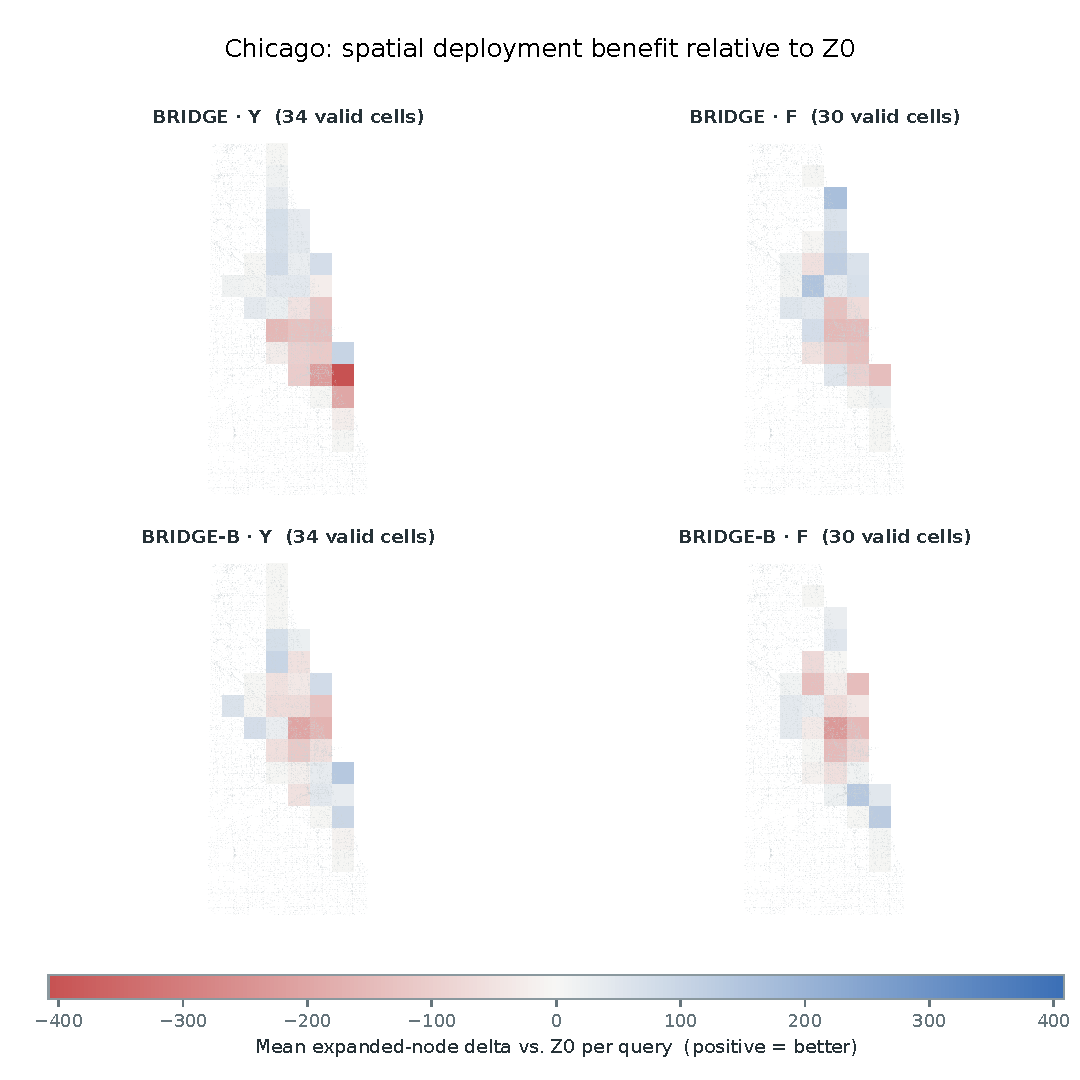
\includegraphics[width=0.9\linewidth]{figures/spatial_benefit_chicago.pdf}
  \caption{Chicago: per-query expanded-node differences of \gmethod{} and \bmethod{}
  against \zmethod{} in $Y$/$F$. Positive and negative cells coexist --- local
  improvements do not add up to a city-wide advantage.}
\end{figure}
\fi

\section*{Data availability}
Raw data come from the public sources cited in the text. The public scope and permanent
links for the processed data, fixed splits, and labels will be added after the license
audit is completed before submission.

\section*{Code availability}
An anonymous reproduction repository and its archival link will be added before
submission.

\section*{Declaration of generative AI and AI-assisted technologies}
During this research and the preparation of the manuscript, the authors used OpenAI Codex
to assist with writing, refactoring, and debugging parts of the research code, tests, and
experiment scripts, and with the structure and language of the article. All code and text
were reviewed, tested, verified, and edited by the authors as needed; the experimental
data come from real program executions, and method selection, result interpretation, and
scientific conclusions were made by the authors. The authors take full responsibility for
the content of the paper.

\section*{Declaration of competing interest}
The authors declare that they have no known competing financial interests or personal
relationships that could have appeared to influence the work reported in this paper.
% TODO: confirm, or replace with the actual declaration.

\section*{CRediT authorship contribution statement}
\noindent Shengyang Xi: Conceptualization, Methodology, Software, Formal analysis,
Investigation, Validation, Visualization, Writing -- original draft, Writing -- review
\& editing, Project administration.\\[0.4em]
Yihan Xiao: Resources, Data curation, Formal analysis, Investigation, Methodology,
Software, Validation, Writing -- original draft, Writing -- review \& editing.\\[0.4em]
Jiawen Wang: Investigation, Software, Validation.

\section*{Funding}
This research received no specific grant from funding agencies in the public,
commercial, or not-for-profit sectors.

\section*{Acknowledgments}
% TODO: fill in.
\noindent\hrulefill

\bibliographystyle{elsarticle-harv}
\bibliography{references}

\end{document}
